\documentclass[12pt]{article}
\usepackage{fancyhdr}
\usepackage{amsmath,amsfonts,enumerate,amssymb}
\usepackage{color,graphicx}
\usepackage{float}
\pagestyle{fancy}
%%%%%%%%%%%%%%%%%%%%%%%%%%%%%%%%%%%%%%%%%%%%%%%%%
% Do your customization here
%%%%%%%%%%%%%%%%%%%%%%%%%%%%%%%%%%%%%%%%%%%%%%%%%
\newcommand{\masunitnumber}{MH4311}
\newcommand{\examdate}{December 2017}
\newcommand{\academicyear}{2017-2018}
\newcommand{\semester}{I}
\newcommand{\coursename}{Cryptography}
\newcommand{\numberofhours}{2}

\newcommand{\ZZ}{\mathbb{Z}}
\newcommand{\CC}{\mathbb{C}}
\newcommand{\RR}{\mathbb{R}}
\newcommand{\FF}{\mathbb{F}}
%\DeclareMathOperator{\diam}{diam}
%%%%%%%%%%%%%%%%%%%%%%%%%%%%%%%%%%%%%%%%%%%%%%%%%
% Don't touch anything from here till instructions
% to candidates
%%%%%%%%%%%%%%%%%%%%%%%%%%%%%%%%%%%%%%%%%%%%%%%%%
\lhead{}
\rhead{}
\chead{{\bf NANYANG TECHNOLOGICAL UNIVERSITY}}
\lfoot{}
\rfoot{}
\cfoot{}
\begin{document}
\setlength{\headsep}{5truemm}
\setlength{\headheight}{14.5truemm}
\setlength{\voffset}{-0.45truein}
\renewcommand{\headrulewidth}{0.0pt}
\begin{center}
SEMESTER \semester\ EXAMINATION \academicyear
\end{center}
\begin{center}
{\bf \masunitnumber\ -- \coursename}
\end{center}
\vspace{20truemm}

\noindent \examdate\hspace{55truemm} TIME ALLOWED: \numberofhours\ HOURS

\vspace{19truemm}
\hrule
\vspace{19truemm}

\noindent\underline{INSTRUCTIONS TO CANDIDATES}
\vspace{8truemm}
%%%%%%%%%%%%%%%%%%%%%%%%%%%%%%%%%%%%%%%%%%%%%%%%%%%%%%
% Adjust your instructions here
%%%%%%%%%%%%%%%%%%%%%%%%%%%%%%%%%%%%%%%%%%%%%%%%%%%%%%
\begin{enumerate}
\item This examination paper contains {\bf FOUR (4)} questions and comprises 
{\bf FOUR (4)} printed pages.

\item Answer all questions. 
The marks for each question are indicated at the beginning of each question.


\item Answer each question beginning on a {\bf FRESH} page of the answer book.

\item This is a {\bf RESTRICTED OPEN BOOK} exam. You are allowed to bring into the examination hall {\bf ONE (1)} piece of A4-size paper written or printed on both sides.

\item Candidates may use calculators. However, they should write down systematically the steps in the workings.
\end{enumerate}

%%%%%%%%%%%%%%%%%%%%%%%%%%%%%%%%%%%%%%%%%%%%%%%%%
% leave this as it is
%%%%%%%%%%%%%%%%%%%%%%%%%%%%%%%%%%%%%%%%%%%%%%%%%
\newpage
\lhead{}
\rhead{\masunitnumber}
\chead{}
\lfoot{}
\cfoot{\thepage}
\rfoot{}
\setlength{\footskip}{45pt}
%%%%%%%%%%%%%%%%%%%%%%%%%%%%%%%%%%%%%%%%%%%%%%%%%%
% put your exam questions here
%%%%%%%%%%%%%%%%%%%%%%%%%%%%%%%%%%%%%%%%%%%%%%%%%%

\paragraph{Question 1.}   Hash function and MAC\hfill (20 marks)
\begin{enumerate}[(a)]
    \item SHA-256 is applied to hash a message with length of 3000 bits. How many compression function operations are needed in the hashing?{\vspace{-1em}\begin{flushright} (5 marks)\end{flushright}}
    \item HMAC-SHA-256 is applied to compute the authentication tag of a message with length of 3000 bits. How many compression function operations are needed?\hfill (5 marks)
    \item At a website, each user's password \textit{P} is hashed together with a salt \textit{S} into a password image \textit{PI}. The password images are stored at the website. Suppose that each salt is a 256-bit random number. The following algorithm is used to hash the password and the salt:\\\\$\begin{aligned}
    t1&=\textit{SHA--}256(P)\oplus S;\\
    t2&=\textit{SHA--}256(t1)\oplus P;\\
    t3&=\textit{SHA--}256(t2)\oplus t1;
\\
t4&=\textit{SHA--}256(t3)\oplus t2;\\
PI&=t3||t4;
    \end{aligned}$\\\\\\
    Is this password hashing algorithm secure? Please justify your answer.{\vspace{-1em}\begin{flushright} (10 marks)\end{flushright}}
\end{enumerate}

\paragraph{Answer}
\begin{enumerate}[(a)]
\item SHA-256: 512-bit block size
\begin{equation*}
3000 + 1 + X + 64=\alpha \cdot 512
\end{equation*}
3000: Bits allocated for message\\
1: 1-bit allocation for start of padding\\
$X$: Number of `0's required for padding\\
64: Length of message stored in 64 bits.\\\\
Solving the equation for the smallest $\alpha$ and $X$ will tell us that
\\$\alpha=6$\\$X=7$\\\\
$\therefore$ 6 compression functions are required\hfill $\square$
\item Note that HMAC uses the following compression function:
\begin{equation*}
MAC_k(M)=Hash((k'\oplus outerpad)||Hash((k'\oplus innerpad)||M))
\end{equation*}
The values of innerpad and outerpad are not required for this question. Instead, you should know that $k'$ is a key that has been padded with `0's to match the block size (i.e. SHA-256: 512-bit block size).\\
$\Rightarrow ((k'\oplus innerpad) || M)$ has size \textbf{3512} bits.\\\\
Hashing 3512 bits using SHA-256 requires us to solve the equation:
\begin{equation*}
3512+1+X+64=\alpha\cdot 512
\end{equation*}
3512: Bits allocated for message\\
1: 1-bit allocation for start of padding\\
$X$: Number of `0's required for padding\\
64: Length of message stored in 64 bits.\\\\
Solving the equation for the smallest $\alpha$ and $X$ will tell us that
\\$\alpha=7$\\$X=7$\\\\
$\therefore$ 7 compression functions are required.\\\\\text{*}Note: The calculation is not complete at this stage.\\\\The output of SHA-256 is 256-bits, as the number implies. For simplification, we shall denote it with $\beta$.\\
$\Rightarrow ((k'\oplus outerpad)|| \beta)$ is $512+256=\textbf{768}$ bits long.\\\\
Hashing 768 bits using SHA-256 requires us to solve the equation:
\begin{equation*}
768+1+X+64=\alpha\cdot 512
\end{equation*}
Solving the equation for the smallest $\alpha$ and $X$ will tell us that
\\$\alpha=2$\\$X=191$\\\\
$\therefore$ 2 compression functions are required.\\\\In total, 9 compression functions are required to hash 3000 bits in HMAC-SHA-256.\hfill $\square$
\item This is a very simple question if you take the effort to rewrite the equations given.\\\\Now, to obtain \textit{P} we can rewrite the equations into the following form.
\begin{equation*}
\begin{split}
P&=t2\oplus \text{SHA--}256(t1)\\
&=t4\oplus \text{SHA--}256(t3)\oplus \text{SHA--}256(t1)
\end{split}
\end{equation*}
We are further told that the salt is a 256-bit random number, which means \textit{S} is 256 bits long. From here, we analyse two equations. Specifically:
\begin{equation*}
\begin{split}
t1&=SHA-256(P)\oplus S\\
t3&=SHA-256(t2)\oplus t1
\end{split}
\end{equation*}
This tells us that both $t1$ and $t3$ are 256 bits long.\\\\The website stores login credentials as a password image $PI$. Assume that $PI$ is $n$ bits long. Since $t3$ is already known to be 256 bits long, $t4$ must be $n-256$ bits long. Note that $PI$ is a mere concatenation of $t3$ and $t4$, which means we have instantly obtained these intermediate values.\\\\We still lack the value of $t1$, crucial for us to compute the value of $P$. Looking at the equations given, we can rewrite the following:
\begin{equation*}
\begin{split}
t3&=\text{SHA--256}(t2)\oplus t1\\
\Rightarrow t1&=\text{SHA--256}(t2)\oplus t3
\end{split}
\end{equation*}
We find that to compute $t1$, $t2$ needs to be obtained. Again, the following equation can be rewritten:
\begin{equation*}
\begin{split}
t4&=\text{SHA--256}(t3)\oplus t2\\
\Rightarrow t2&=\text{SHA--256}(t3)\oplus t4
\end{split}
\end{equation*}
From this point, we can obtain the values of $t2$ and $t1$. Note that the SHA-256 values can easily be calculated by using a program (as the algorithm is standardised). Substituting the respective values will now allow us to obtain $P$ in its plaintext form. This demonstration shows you that this algorithm is extremely insecure (and the little effort required from an attacker to obtain passwords).\hfill $\square$
\end{enumerate}
\paragraph{Question 2.}   AES\hfill (15 marks)
\begin{enumerate}[(a)]
\item In AES, the irreducible polynomial with binary coefficients, $x^8+x^4+x^3+x+1$, is used to define $GF(2^8)$. Find the inverse of 5 in this field.{\vspace{-1em}\begin{flushright} (10 marks)\end{flushright}}
\item Suppose that you are required to implement AES to encrypt files on your computer. The encryption and decryption is provided by the user. When a user inputs the decryption key, your program should check whether the key is correct or not, and the decryption is performed only when the key is correct. Briefly explain how to implement it.\hfill (5 marks)
\end{enumerate}
\paragraph{Answer}
\begin{enumerate}[(a)]
\item 
\textbf{NEVER attempt AES calculation questions in decimal form. Always convert to polynomial form first!}\\\\
5 in the field $GF(2^8)$ is expressed as the polynomial $x^2+1$. Calculate the inverse as follows:
\begin{equation*}
x^8+x^4+x^3+x+1\mod x^2+1=(x^6+x^4+x)(x^2+1)+1
\end{equation*}
$\therefore (x^2+1)^{-1}=(x^6+x^4+x)$.\\
$x^6+x^4+x$ converted to hex(adecimal) form is \{52\}.\hfill $\square$
\item Hash the key and store the digest together with the ciphertext.\hfill $\square$
\end{enumerate}
\paragraph{Question 3.}   RSA\hfill (20 marks)
\begin{enumerate}[(a)]
\item In a toy RSA encryption scheme, the public key $(n,e)$, the private key is $d$. It is given that $n=3149=47\times 67$. You are required to generate a pair $(e,d)$. \hfill (10 marks)
\item Factorise $n=84923$ using the following relations:\hfill (10 marks)\\
\begin{equation*}
\begin{split}
345^2\mod n&=2\times 17^2\times 59\text{ ;}\\
513^2\mod n&=2^4\times 3\times 5\times 7\text{ ;}\\
519^2\mod n&=2^8\times 3\times 19\text{ ;}\\
520^2\mod n&=7^2\times 11\times 29\text{ ;}\\
527^2\mod n&=2^6\times 3\times 5^2\times 7
\end{split}
\end{equation*}
\item In an RSA implementation, the random number used in OAEP is generated by applying SHA-256 to hash the plaintext. Is this implementation secure? Please justify your answer.\hfill (10 marks)
\item The decryption of a toy RSA is implemented on a computational device. The private key $d$ is 10-bit. Right-to-left square-and-multiply algorithm is used in the implementation. Chinese remainder theorem and RSA blinding are not used in the implementation. During the decryption, the electrical current consumed by the device is measured and is shown in the following diagram (the horizontal axis is time, the vertical axis is the electrical current). What is the value of $d$? Briefly explain how you obtain the value of $d$. \hfill (10 marks)
\begin{figure}[H]
\centering
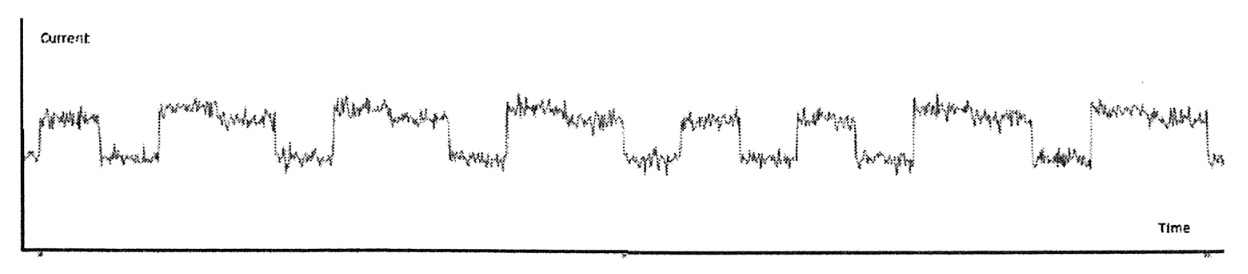
\includegraphics[width=1\linewidth]{Capture}
\label{fig:capture}
\end{figure}
\end{enumerate}
\paragraph{Answer}
\begin{enumerate}[(a)]
\item \begin{equation*}
\begin{split}
n&=p\times q\\
&=47\times 67\\
\varphi(n)&=(p-1)(q-1)\\
&=46\times 66\\
&=3036
\end{split}
\end{equation*}
We have obtained $\varphi(n)$ and so take $e$ to be 5.
\begin{equation*}
\begin{split}
\gcd(\varphi(n),e)&=1\\
\text{(Check) }\gcd(3036,5)&=1
\end{split}
\end{equation*}
Now calculate for the value of $d$.
\begin{equation*}
\begin{split}
ed&\equiv 1\mod \varphi(n)\\
3036&=607\times 5+1\\
\Rightarrow 1&=3036-607\times 5\\
\because d&=e^{-1}\\\therefore d&=5^{-1}\\&=-607\\&=2429\mod 3036
\end{split}
\end{equation*}
For $n=3149$, we can take a pair $(e,d)$ as $(5,2429).$\hfill $\square$
\end{enumerate}
\newpage
\paragraph{Question 4.}   Digital Signature Algorithm\hfill (25 marks)
\begin{enumerate}[(a)]
    \item A 96-bit private key is used in the Digital Signature Algorithm. Please develop an efficient attack to break it.\hfill (10 marks)
    \item In the Digital Signature Algorithm, what is the risk if the same random number is reused to sign different messages?\hfill (5 marks)
    \item In the Digital Signature Algorithm, the random number used to sign message \textit{M} is generated by applying SHA-256 to hash the key together with the message digest of M. Is this implementation of the Digital Signature Algorithm secure? Please justify your answer.{\vspace{-2.5em}\begin{flushright} (10 marks)\end{flushright}}
\end{enumerate}
\bigskip
\vfill
\begin{center}{\bf END OF PAPER}\end{center}
\end{document}
